\newcommand{\ClassPath}{../../VIU_TFM_LaTeX_template}
\documentclass{\ClassPath/viu-tfm-template}
\usepackage{multicol}

\definecolor{maincolor}{HTML}{f25416}

%--------------------------------------------------------------------------
% Definiciones necesarias Modifica con tus datos
%--------------------------------------------------------------------------
\def\nombre{Gómez Olivencia, Rubén}
\def\dni{78910013-A}
\def\titulo{Implementación de validaciones \linebreak\linebreak del lado del servidor con Laravel}
\def\titulacion{Máster Universitario en Desarrollo de Aplicaciones y Servicios Web}
\def\curso{2022-2023}

%Los siguientes son opcionales: si no se ponen, la portada cambia un poco. Ideal para escribir artículos/trabajos cortos
\def\dirige{}
\def\convocatoria{}
\def\asignatura{Seguridad Web}


% importar fichero de Bibliografía
%\addbibresource{Actividad_1.bib}

\begin{document}
\graphicspath{{../../VIU_TFM_LaTeX_template/}}

\coverpage

\tableofcontents

\chapter{Introducción}

La seguridad en un proyecto informático es algo que se debe pensar desde el inicio de un proyecto, ya que las decisiones tomadas pueden repercutir en las iteraciones posteriores y en la evolución del producto que estemos realizado.

A lo largo de este documento se van a explicar las decisiones tomadas, tanto en el ámbito de programación como de diseño, durante la creación de un formulario de registro para un portal web creado con el \textit{framework} \href{https://laravel.com/}{Laravel}.


\chapter{Laravel}

Laravel es un \textit{framework} desarrollado en el año 2011 que hace uso del lenguaje de programación \href{https://www.php.net/}{PHP} para la creación de desarrollos basados en la tecnología web.

La idea de todo \textit{framework} es la de crear un entorno de trabajo que unifique distintos conceptos, prácticas y criterios que sirvan como referencia para la creación de un proyecto.

Una de las muchas ventajas que nos proporciona Laravel es la de un sistema modular para la creación de validaciones en formularios, tal como nos indica su \href{https://laravel.com/docs/6.x/validation}{documentación}.

\chapter{Despliegue de la aplicación}
Antes de entrar en detalle en cómo se ha desarrollado la aplicación es importante conocer cómo podemos realizar el despliegue de la aplicación, ya sea para utilizarla o para realizar modificaciones sobre la misma.

\section{Servicios Docker}
Para realizar el desarrollo del proyecto se ha utilizado servicios a través de contenedores \textbf{\href{https://www.docker.com/}{Docker}}, los cuáles pueden ser levantados gracias al fichero \configfile{compose.yaml} y el comando \commandbox{docker-compose up}

Al levantar los servicios con el comando \textbf{docker-compose up} se hará uso de los siguientes puertos:
\vspace{-1em}
\begin{itemize}
    \item \textbf{80}: Para el entorno web, usando Nginx como servidor web.
    \item \textbf{3306}: Para la base de datos.
    \item \textbf{3307}: Para el acceso web a phpmyadmin.
\end{itemize}
\vspace{-1em}

Para el correcto funcionamiento del contenedor se hace uso del fichero \configfile{vhost.conf} que modifica la configuración del servicio Nginx para que funcione de manera correcta con Laravel.

\section{Despliegue del código fuente}
Para realizar el despliegue del código fuente sobre el contenedor del servicio web, el directorio \configdir{src} debe estar situado a la misma altura del fichero \configfile{compose.yaml}.

De esta manera, a la hora de levantar el servicio se crea un volumen compartiendo el directorio local \configdir{src} con otro dentro del contenedor, en la ruta \configdir{/app}, que es de donde se nutre Nginx.


\section{Creación de la base de datos}

El servicio de MySQL se encarga de crear una base de datos llamada \textbf{actividad1} en el momento en el que el servicio se levanta. También crea los siguientes credenciales de acceso a dicha base de datos:

\vspace{-1em}
\begin{itemize}
    \item usuario:  \textbf{actividad1}
    \item contraseña:  \textbf{4ct1v1d4d1}
\end{itemize}
\vspace{-1em}

\section{Despliegue de datos}
Para realizar el despliegue de datos, se va a utilizar dos características que tiene Laravel y que tienen que ver con el despliegue en la base de datos:

\vspace{-1em}
\begin{itemize}
    \item \textbf{Migrate}: Es una forma de tener un sistema de control de versiones del esquema de base de datos. De esta manera, se puede hacer evolucionar el esquema (tablas, columnas, índices, ...) a lo largo del tiempo y también volver a un punto anterior del mismo.
    \item \textbf{Seeds}: También conocido como “semillas”, nos posibilita añadir datos a las tablas que hemos creado. Normalmente se utiliza para crear datos al inicio del proyecto con datos que deben existir (o también datos de pruebas) para que se pueda utilizar el proyecto.
\end{itemize}
\vspace{-1em}

Para realizar el despliegue debemos conectarnos al contenedor donde tenemos el proyecto y lanzar los comandos que realizan el “migrate” y crean los datos. A continuación aparecen los comandos:

\begin{mycode}{Acceder al contenedor Docker para hacer el despliegue}{console}{}
# nos conectamos al contenedor
ruben@vega:~$ docker exec -it   actividad_1_php_1 /bin/bash

# vamos al directorio donde está el desarrollo
root@a7913ac7b97a:/# cd /app

# lanzamos el migrate
root@a7913ac7b97a:/app# php artisan migrate

#lanzamos el seed
root@a7913ac7b97a:/app# php artisan db:seed

\end{mycode}



\chapter{Desarrollo realizado}

Una vez tenemos realizado el despliegue, se va a profundizar en el desarrollo realizado, destacando los siguientes aspectos:

\section{Sistema de autenticación en Laravel}
Laravel cuenta con un sistema de \href{https://laravel.com/docs/6.x/authentication}{autenticación} que nos permite la creación de usuarios de manera sencilla y también gestionar el contenido de las vistas dependiendo de si el usuario ha realizado \textit{login} o es un invitado.

Aparte, gracias al sistema de \textit{\href{https://laravel.com/docs/6.x/frontend}{frontend scaffolding}}, podemos crear las típicas vistas de registro de usuario, login, reseteo de contraseñas, etc., de manera automática, pudiendo elegir entre tres frameworks: \href{https://getbootstrap.com/}{Bootstrap}, \href{https://vuejs.org/}{Vue} o \href{https://es.reactjs.org/}{React}.

Este sistema de autenticación ha sido modificado para que sea más seguro y realizando modificación en los campos que se piden durante el registro.


\subsection{Seguridad durante el login}
Una de las medidas de seguridad más sencilla de implementar es la de no dar información de más cuando existe algún error durante el login de un usuario.

Si un atacante consigue un listado de posibles e-mails que pertenecen a nuestra aplicación, si al intentar el login se le indica que esa cuenta no existe, pasará a realizar el ataque con otra cuenta. Mientras que si no se le indica nada, no obtendrá información y por tanto es posible que intente seguir con la misma cuenta más tiempo.

\begin{center}
    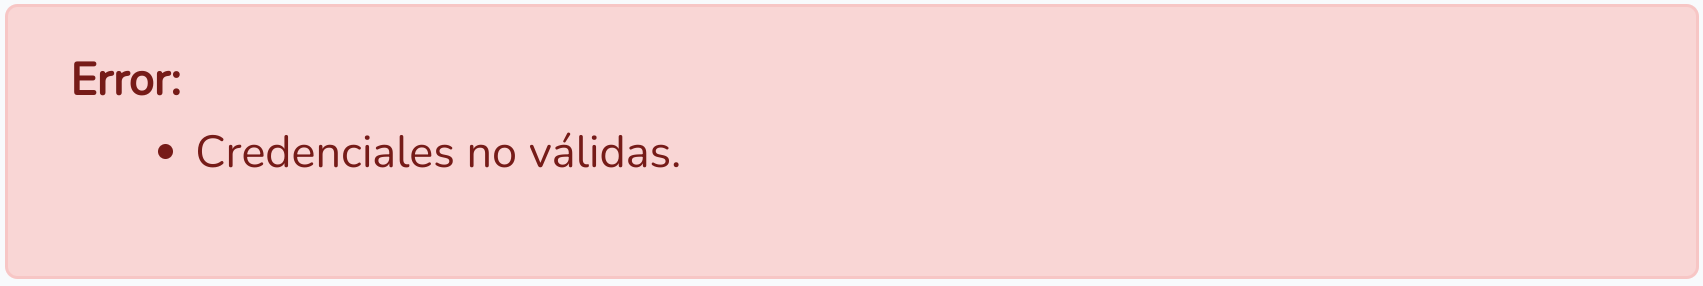
\includegraphics[width=0.8\linewidth]{img/error_simple.png}
\end{center}

Para mostrar este mensaje se ha creado un template en \configfile{resources/views/layouts/_errors.blade.php} que genera el listado visto previamente.

Por otro lado, para no dar pistas también se ha modificado el fichero \configfile{resources/views/auth/login.blade.php} quitando los bordes rojos que aparecen por defecto indicando si el error se ha producido en el login o en la contraseña.


\subsection{Bloqueo de cuentas por fallos de autenticación}
Para asegurar que no se realiza un ataque por fuerza bruta  de contraseñas  Laravel permite el bloqueo una vez realizado un número de intentos fallidos. Por defecto la configuración se encuentra en el fichero \configfile{Illuminate/Foundation/Auth/ThrottlesLogins.php} dentro del directorio \configdir{vendor/laravel/framework/src/}, donde aparece que el número máximo de intentos es de 5 y el bloqueo se efectuará durante 1 minuto.

Para ajustar esta configuración a nuestras necesidades, se ha modificado el fichero \configfile{app/Http/Controllers/Auth/LoginController.php} en el que añadiremos las variables \mintinline{php}{$decayMinutes} y \mintinline{php}{$maxAttempts} quedando:

\begin{mycode}{Añadiendo seguridad durante el login}{php}{}
<?php
...
class LoginController extends Controller
{
    use AuthenticatesUsers;
    protected $redirectTo = RouteServiceProvider::HOME;

    //variables modificadas por seguridad
    public $decayMinutes = 180;
    public $maxAttempts = 2;
...
\end{mycode}

De esta manera, si se intenta hacer login con una cuenta existente y se falla la contraseña 2 veces, se bloqueará el acceso apareciendo el siguiente error:

\begin{center}
    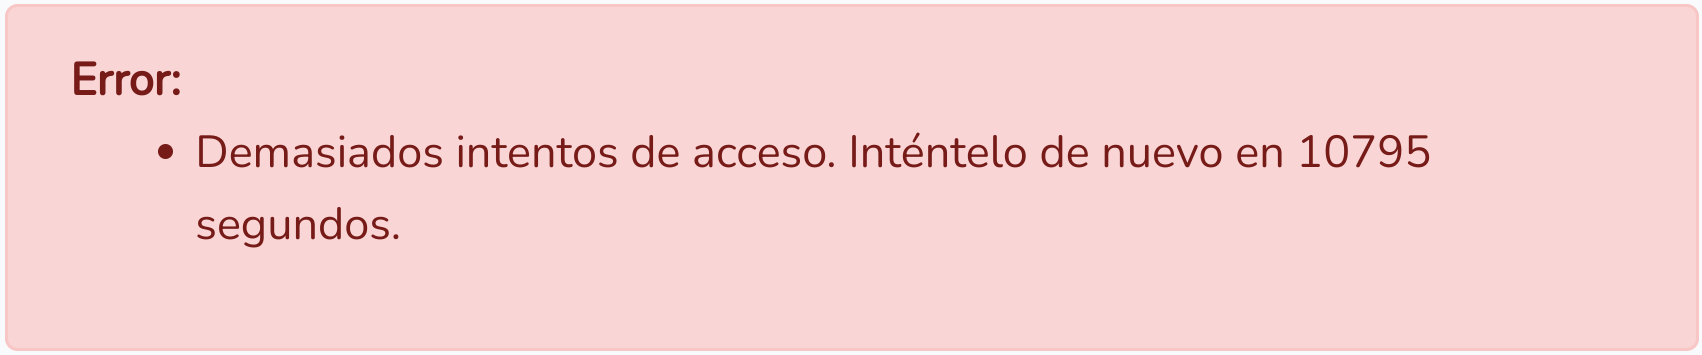
\includegraphics[width=0.8\linewidth]{img/bloqueo.png}
\end{center}

Tal como aparece en el mensaje, ha habido demasiados intentos de acceso fallidos y habrá que esperar un número de segundos (los 180 minutos indicados en la configuración).



\section{Sistema de validación durante el registro}
A la hora de registrarse en una plataforma, hay que asegurarse que los datos introducidos son válidos. Esta validación no sólo se debe realizar en el frontend, ya que ese sistema es fácilmente traspasable con unos mínimos conocimientos.

Los datos deben de validarse antes de acceder a la base de datos, y por tanto se debe de realizar en el \textit{\textbf{backend}} de la aplicación web.

Como ya se ha dicho previamente, Laravel cuenta con una \href{https://laravel.com/docs/6.x/validation}{documentación extensa} acerca de su sistema de validación indicando cómo lo podemos ampliar para adecuarlo a nuestras necesidades, tal como veremos a continuación.

\subsection{Creación de campos propios}
El sistema de registro de Laravel (a través del sistema de autenticación citado previamente) crea una página donde se puede insertar nombre, e-mail y contraseña.

Para añadir nuevos campos debemos modificar el fichero de la vista \configfile{resources/views/auth/register.blade.php} y añadir los campos que nos interese.

Modificaremos \configfile{app/Http/Controllers/Auth/RegisterController.php} para que estos campos posteriormente se inserten en la base de datos, quedando la función \textit{\textbf{create}} de la siguiente manera:


\begin{mycode}{Código para la creación de usuario }{php}{}
<?php
...
protected function create(array $data) {
    return User::create([
        'name'      => $data['name'],
        'surname'   => $data['surname'],
        'dni'       => $data['dni'],
        'email'     => $data['email'],
        'password'  => Hash::make($data['password']),
        'telephone' => $data['telephone'],
        'iban'      => str_replace(' ','',$data['iban']),
        'about'     => $data['about'],
        'country_id'=> $data['country_id'],
    ]);
}
\end{mycode}



\subsubsection{Modificación de la base de datos}
Para que los cambios del paso anterior funcionen, lógicamente hay que realizar la modificación de la base de datos para aceptar los nuevos campos.

Para ello se ha creado un fichero \textbf{\textit{migrate}} en el que se indica  los nuevos campos que se deben añadir a la tabla \textbf{users}.


\subsection{Reglas propias de validación}
Con los nuevos campos creados en la base de datos y con el formulario modificado, es momento de realizar las validaciones oportunas, paso previo a la inserción de datos en MySQL.

Laravel nos permite realizar validaciones sencillas teniendo en cuenta el campo, el tipo de datos, longitud...

\begin{mycode}{Validaciones realizadas}{php}{{\footnotesize }}
<?php
...
protected function validator(array $data)
{
    return Validator::make($data, [
        'name'      => ['required', 'string', 'between:2,20'],
        'surname'   => ['required', 'string', 'between:2,20'],
        'dni'       => ['required', new dni,'max:9'],
        'email'     => ['required', 'email:filter', 'max:255', 'unique:users'],
        'password'  => ['required', 'string', 'min:12', new password, 'confirmed'],
        'telephone' => ['nullable', new telefono,'max:13'],
        'iban'      => ['required', new iban, 'max:24'],
        'about'     => ['nullable', 'string', 'between:20,250'],
        'country_id'=> ['nullable', 'integer']
    ]);
}
\end{mycode}

En las validaciones expuestas, se han realizado validaciones propias para los campos \textbf{dni}, \textbf{password}, \textbf{teléfono} e \textbf{IBAN}. Estas validaciones propias se han creado dentro del directorio \configdir{app/rules}, donde cada fichero es una validación y contienen una clase con dos funciones principales:

\begin{itemize}
    \item \textbf{passes}: función que recibe el contenido del campo del formulario y en el que realizaremos la validación. Las validaciones realizadas para este proyecto se han solucionado con una o varias expresiones regulares.

    \item \textbf{messages}: devuelve el mensaje de error en caso de que la función “passes” \textbf{no devuelva true}.
\end{itemize}

En caso de que existan varios mensajes de error, aparecerán todos seguidos e indicando cuáles son los campos que han dado error, a través de un borde rojo:

\begin{center}
    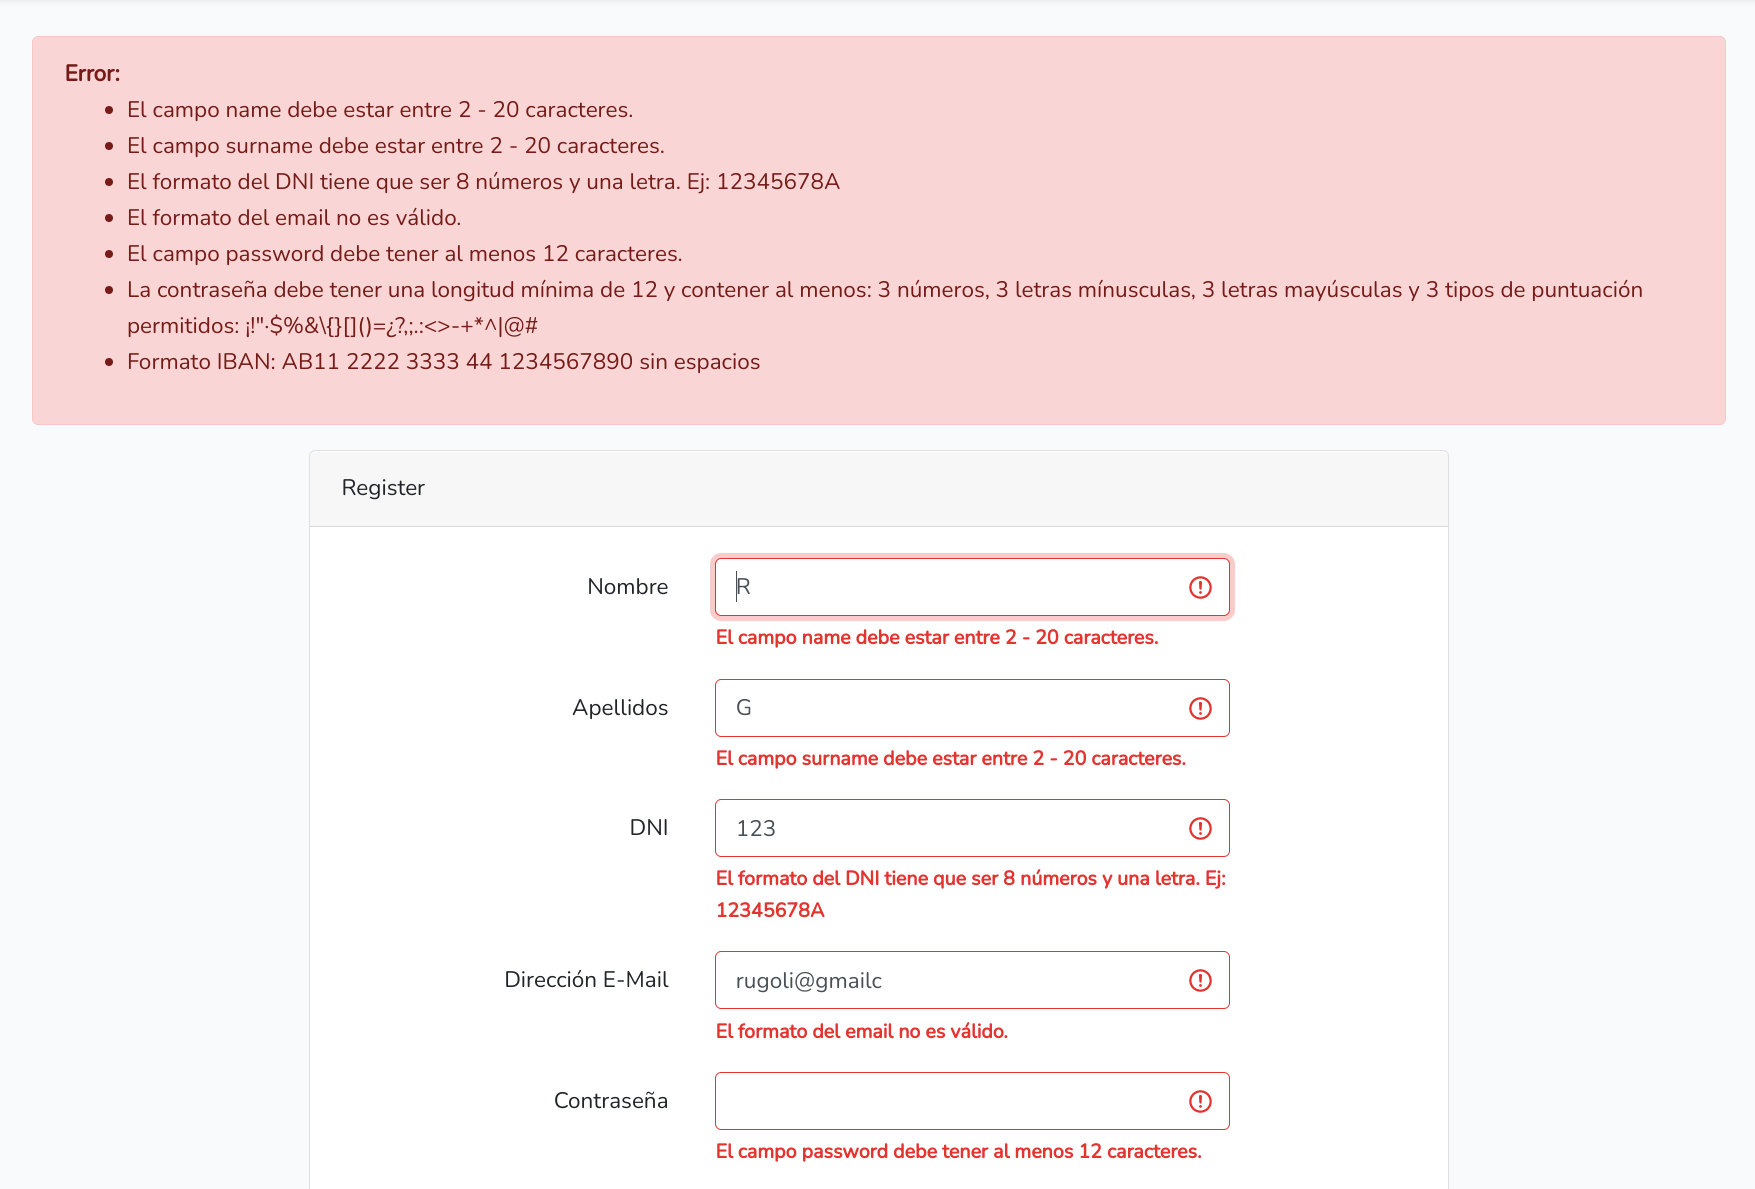
\includegraphics[frame,width=0.8\linewidth]{img/errores.png}
\end{center}


Una de las validaciones más importantes realizadas ha sido la de la contraseña, la que se ha forzado que tenga que ser:

\begin{itemize}
    \item Al menos 10 caracteres, de los cuales:
    \item Al menos 2 tienen que ser letras minúsculas.
    \item Al menos 2 tienen que ser letras mayúsculas.
    \item Tiene que haber al menos 2 números.
    \item Tiene que incluir al menos 1 símbolo tipográfico.
\end{itemize}

Esta validación se ha conseguido mediante expresiones regulares en su fichero de reglas propio. De cara a futuro, se podría mejorar creando unas variables de entorno en el fichero \configfile{.env} donde se indique el la dificultad de la contraseña a introducir.

\subsection{Mantener valores en el formulario tras un error}
Tal como se ha visto en el paso anterior, en caso de que el registro devuelva un error durante la validación, se le indicará al usuario, indicando los campos que debe corregir.

Es por eso que es importante mantener los valores que ha introducido previamente, ya que de esta manera estaremos facilitando la usabilidad de la aplicación.

Esto se ha conseguido en la vista del registro indicando en los parámetros \textit{\textbf{value}} el valor previo que nos permite obtener Laravel.


\begin{mycode}{Valores antiguos en el formulario}{html+php}{}
<input id="dni" type="text" class="form-control
    @error('dni') is-invalid @enderror" name="dni"
    value="{{ old('dni') }}"
    required autocomplete="dni" autofocus>
\end{mycode}

Esto se ha repetido para todos los campos, a excepción de la contraseña.

\subsection{No permitir “copiar-pegar” en la contraseña}
Para mejorar la seguridad y evitar que algún atacante, mediante ingeniería social delante del ordenador, pueda copiar la contraseña introducida, se han modificado los campos de contraseña y validación de contraeña para no permitir copiar, seleccionar o pegar contraseña.

No permitiendo “copiar-pegar” también nos estamos asegurando que el usuario introduce de manera correcta la contraseña que ha elegido, minimizando el riesgo de equivocarse.

\begin{mycode}{No permitimos “copiar-pegar” en el input}{html+php}{}
<input id="password" type="password" class="form-control
    @error('password') is-invalid @enderror"
    name="password" required autocomplete="new-password"
    onselectstart="return false"
    onpaste="return false;"
    onCopy="return false"
    onCut="return false"
    onDrag="return false"
    onDrop="return false"
    autocomplete=off/
>
\end{mycode}

Con el código expuesto, evitamos copiar, cortar, seleccionar, arrastrar y pegar el contenido de los textos que serán guardadas como contraseñas.

\section{Traducciones}
Tal como se ha visto en la imágenes, los mensajes de validación aparecen en castellano, ya que se han añadido traducciones de los mensajes originales y porque la aplicación ha sido configurada con el castellano como idioma principal.

Las traducciones de los mensajes se han añadido en el directorio \configdir{resources/lang/es}, manteniendo la misma estructura de ficheros existente en el idioma inglés.

Para realizar parte de las traducciones se ha utilizado como base las traducciones ya realizadas por Marco Gomes de su \href{https://github.com/MarcoGomesr/laravel-validation-en-espanol}{proyeto de GIthub}.

Las traducciones para los campos propios del proyecto se han añadido al fichero \configfile{formulario.php} dentro del directorio indicado previamente.

\vfill
\pagebreak

\chapter{Conclusiones}
Hoy en día es habitual que en cualquier portal web de servicios haya que realizar un registro con ciertos datos personales. Es importante que estos datos sean validados y que se compruebe que la seguridad del portal no se ve comprometida por los datos introducidos.

Es por eso que, previa a la inserción de los datos en la base de datos, es obligatorio realizar una validación de los datos introducidos en los formularios, tal como hemos visto a lo largo de este documento.

Aunque de primeras quizá pueda parecer una labor tediosa, los framework como Laravel facilitan esa labor. Por eso no hay excusa para no hacer uso de estos sistemas de validaciones, que por otro lado también ayudan al usuario a utilizar nuestras aplicaciones mejorando la usabilidad de la misma.



\end{document}
